%!TEX root = /Users/smsohan/Taggy/Thesis/ucalgthes1_root_0.tex
\fancyhead[RO,LE]{\thepage}
\fancyfoot{} 
\chapter{Taggy}
\label{ch:taggy}
In this chapter, I have presented the details of my auto-tagging technique in terms of Taggy. Taggy is a prototype implementation of the technique. First, the underlying assumptions behind Taggy are discussed. Then, a definition of the adapted agile project context is given. With this background information, a high level architecture of Taggy is explained. Next, the workflow of auto-tagging is discussed. The mathematical and algorithmic details are provided in the similarity computation section. This chapter also includes the details about the software frameworks used to implement Taggy. Finally, an illustrative example is given to explain Taggy in action.

\section{Assumptions}
Taggy is designed to auto-tag the emails with user stories based on the following assumptions:

\begin{enumerate}
	\item An email is potentially relevant to a user story when:
		\begin{itemize}
			\item It is sent during the iteration time frame of the user story. Since agile projects are developed in small iterations and the core concentration during an iteration is to deliver the user stories from the iteration backlog, it is highly likely that the email conversation will be about the user stories from current iteration backlog. However, it is also possible to see some conversations about near past or near future iteration backlogs. Such conversation are mainly used to provide post-delivery feedback and collaborate about upcoming work. Taggy uses this assumption to shorten its search space for relevant user stories by filtering out the ones from long ago.
			
			\item The developers and/or customers of a user story often communicate via email. For an example, if Alex (a developer) is working on a user story for Jane (the customer), and Alex writes an email to Jane, they are more likely to discuss about the user story than Peri (another developer) and Jane. However, Peri can always participate in a discussion about Alex's work in an agile team, where open communication is encouraged. But, it is highly unlikely that two people who are neither assigned developers or customers of a user story will write emails about that. This assumption about people's participation in email provides an important clue for Taggy's similarity computation.
			
			\item There is a minimum degree of text similarity between an email and a user story. An email has text in terms of its subject, body and attachments. Although not explicit, it is likely that such text in the emails will show some relevance to the user stories. This may not be true in all cases, especially if there is a lot of face-to-face communication. However, this is not the case for distributed projects with huge time zone difference. Taggy computes a text similarity between the email and user story and discards the ones that show very poor match.
		\end{itemize}
	 \item A web-based project management tool is used to manage the distributed agile project. To automatically link up emails with user stories, Taggy looks into this tool for information about user stories. This assumption is required because if teams only use low-fi physical artifacts, such as sticky notes for user stories on a whiteboard, it is not possible to automatically find the user stories. As discussed in Chapter~\ref{ch:related_work}, distributed agile teams use a number of different types of such tools.
	
	\item The project management tool captures user stories with its planning information including a) assigned developers, b) customer and c) iteration timeframe. The presence of this planning information is essential as it serves as the meta data that is necessary to auto-tag emails. While it is generally expected that this data be available, it is not required that each and every user story contains all the required planning information. Since Taggy uses context alongside text similarity, having the context helps in making a more informed decision in auto-tagging.
	
	\item Each project has its own email address termed as ``project email'' so that when people are sending emails about a project to someone, they can keep the project's email in the copy. This serves as the input to Taggy for auto-tagging. Also, giving every project a unique email address ensures Taggy can correctly determine the target project for an email. Since most people who use email are already familiar with the CC: feature, this adds little learning curve or communication overhead. It is assumed that indicating the project in CC: serves a convenient input mechanism compared to manually copy-pasting the email contents into a system for every useful email.		
	
	\item The subject of an email carries an important clue about its relationship with a user story. Although, subject line is just text, similar to the body or attachment contents of an email, due to professional etiquette and for the sake of grabbing attention, people write informative subjects when writing emails about projects. Taggy distinguishes the text relevance of the subject from the rest of the email contents based on this assumption.
\end{enumerate}



\section{The Agile Project Context}
Taggy uses two kinds of context information that are available for agile user stories, namely Temporal context and People context. These contexts are defined below:

\begin{enumerate}
	\item \textbf{Temporal Context.} User stories in agile projects are grouped by small iterations so that a bunch of new user stories are potentially shippable at the end of each iteration. These iterations are confined within specific start and end dates. This time-box works as the temporal context for a user story. For example, if a user story is developed during Iteration\#2, June 1 to June 14, then Taggy assumes people are more likely to write emails about the user story within this period than in the far past or future.
	
	\item \textbf{People context.} The people context for a user story is formed by its assigned developers and customers. A user story may have one or more customers who are mainly responsible for providing the details proactively and as questions arise during implementation. On the other hand, a user story is broken down into tasks and assigned to developers, testers and other technical team members. Taggy uses all the people relevant to a user story as its people context. For example, if an email is exchanged among the people in a user story, then Taggy puts a higher similarity rank than when the people context is different. The identification of the people context is done based on email addresses. The people context for an individual can include multiple email addresses.	
\end{enumerate}

Since Taggy combines context similarity with text similarity, the above contexts provide more information for auto-tagging. However, when some or all of the context information are missing for a user story, Taggy still applies whatever information is available to auto-tag emails with user stories.

\section{High Level Workflow}
Taggy is designed to be used in a live system as illustrated in Figure~\ref{fig:workflow}. The following list explains each step of the workflow: 
\begin{figure*}[!h]
	\centering
	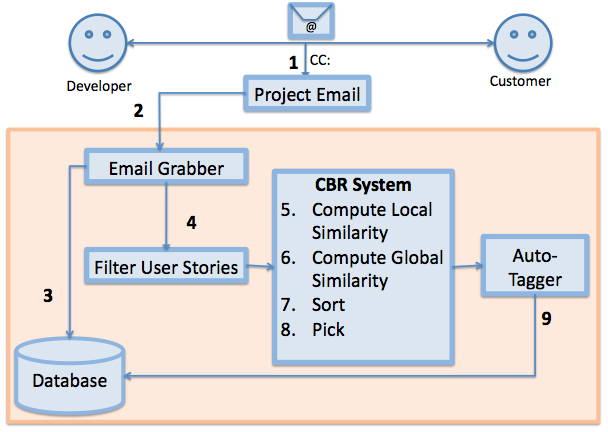
\includegraphics[width=\textwidth]{workflow.png}
	\caption{Email Auto-tagging Workflow}
	\label{fig:workflow}
\end{figure*}

\begin{enumerate}
	\item \textbf{Copy emails to project email address.} This is the input step for Taggy. As discussed in the assumptions, Taggy identifies each project by its own email address. So, whenever someone sends an email about a project, they put the ``project email'' in the CC:. This is the only change in the business process that needs to be implemented by the distributed team. This intake process was successfully adapted in previous work \cite{where_did_you}. In case someone forgets to do this while sending the email, it is possible to simply forward the email to the ``project email'' later.
	
	\item \textbf{Grab email.} Once the project related emails reach the inbox of ``project email'', Taggy picks up the email. It is common for email servers to allow access via POP or IMAP protocol. Taggy uses POP3 to read all incoming emails, including the attachments, if any. This grabbing runs on a background process, which can be scheduled to check for new emails in desired intervals. However, this email-grabbing step can make use of any other email transfer protocol.

	\item \textbf{Save email.} After grabbing, Taggy saves the email into its database, keeping a link to its project. After this step, even if auto-tagging fails, the email is still stored under the project. This step makes an email available for search and browsing without the need for looking into other users' inboxes.
	
	\item \textbf{Filter.} To auto-tag the email just grabbed, Taggy first reduces its search space by discarding the user stories of a project that were done in the far past or scheduled to be developed in the far future. This is because comparing against all user stories is too slow if a project has a lot of user stories from far past or future. This filtering process essentially finds the current iteration of the project, if any. Then, it considers the user stories from the current iteration and its neighboring iterations in a month as potential candidates for auto-tagging the emails. In the evaluation data sets, I have found 95\% of the emails were sent during this time period. However, this heuristic will fail if an email is actually sent about a user story from far past or future iteration.

	\item \textbf{Compute local similarity.} In the reduced search space, Taggy computes local similarities for people and temporal contexts as well as separate text similarities for subject and body. The details of these local similarity computations are discussed in Section~\ref{sec:equations}.
	
	\item \textbf{Compute global similarity.} Next, for each of the user stories, the similarity values from previous step are combined to produce a global similarity score. This computation is done based on the formula presented at Equation~\ref{eq:global} . This global similarity assigns a numeric value of the relative relevance between a user story and the email.
	
	\item \textbf{Sort.} The user stories are then sorted descendingly according to their global similarity value from previous step. This produces a list of user stories with the potentially most relevant user story at the top.
	
	\item \textbf{Pick.} Next, Taggy picks the user stories having global similarity scores above a predefined threshold. Having a threshold ensures Taggy only picks the ones that show sufficient relevance based on its learning. However, this also means that for some emails no user story may be picked. Instead of picking up all the user stories above threshold, Taggy can be configured to pick up only the top n stories, where n is a number greater than or equal to one. This allows Taggy to limit the auto-tagging to a limited number of user stories per email. Selecting a large value of n may produce false positives where a small value may produce false negatives. The same trade-off exists with the threshold selection as well. The value of n can be determined based on the historical data so that n equals the average number of user stories that are discussed per email. Similarly the threshold score can be set by looking at the historical data.
	
	\item \textbf{Auto-tag.}	Finally, Taggy auto-tags the email with the picked user stories from the last step. This step adds database level links between the email and the user stories to be auto-tagged.
\end{enumerate}

However, to auto-tag instant messages, steps 1-3 of the aforementioned steps differ significantly. Figure~\ref{fig:im_intake} shows these three steps. These new steps are explained next:

\begin{figure*}[!h]
	\centering
	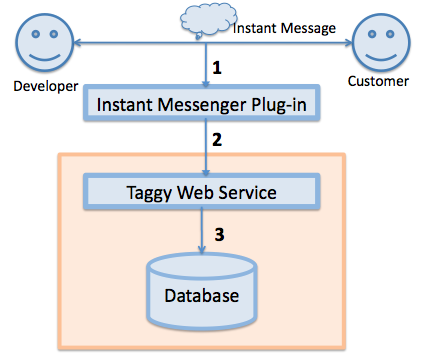
\includegraphics[width=0.6\textwidth]{im_intake.png}
	\caption{Taggy Instant Message Intake Process}
	\label{fig:im_intake}
\end{figure*}


\begin{enumerate}
	\item \textbf{Activate instant message plugin.} Instant message clients often allow the use of plugins. For example, Skype \cite{skype} has a plugin framework and Taggy has a plugin for Skype. To input the instant messages, one needs to activate the Taggy plugin and select the project under discussion. Then, as the chat messages are exchanged, the plugin sends out the messages to Taggy over a web-based service. Typically the instant message clients provide meta data such as unique identification of a chat session, its individual messages, people involved and also the time stamp.

	\item \textbf{Grab instant message.} Taggy exposes a web service for the intake of instant messages. As soon as it finds a chat message from the plugin, it identifies the conversation based on the meta data.
	
	\item \textbf{Save instant message.} Taggy extracts out the context from an instant message and saves it in the database. For example, it matches the instant message identifier for people that are already stored in the database against the ones participating in a chat session. Also, it keeps track of the time stamp. As a result, an instant message is stored with a similar people and temporal context as that of an email. Instant messages that are part of a single conversation are stored together in Taggy. The conversation is identified by the supplied identifier from instant messaging client.
\end{enumerate}

Since instant messages don't capture any subject, Taggy cannot produce a subject similarity. As a work around for this limitation, Taggy can be trained differently for instant messages where the contribution of subject similarity is ignored.

On a live system, as like any other machine learning solution, Taggy cannot discard the possibility of a wrong auto-tagging decision. When someone spots such a faulty auto-tagging in Taggy, she/he can manually correct it.

However, similar to most machine learning techniques, Taggy needs to learn some parameters before it is ready for use. Figure~\ref{fig:learn_evaluate} shows the two high level steps involved in the process of learning the relative weights of similarity measures. 

\begin{figure*}[!h]
	\centering
	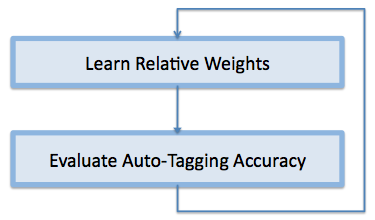
\includegraphics[width=0.5\textwidth]{learn_evaluate.png}
	\caption{Taggy High Level Workflow}
	\label{fig:learn_evaluate}
\end{figure*}

The details of finding a set of initial relative weights and learning is discussed later in Section~\ref{sec:learning}. Once the weights are learned, the system needs to be evaluated to see its accuracy. Based on the findings of evaluation, the learning is reiterated to find a set of relative weights that produces optimum auto-tagging accuracy. This process is discussed in greater detail in Chapter~\ref{ch:evaluation}.

\section{Similarity Computation}
As it is shown in the workflow, a similarity computation function forms the heart of Taggy. This is performed using a machine learning technique called Case Based Reasoning (CBR). A CBR system is implemented to find out relevant user stories for an email or instant message. 

\begin{figure*}[!h]
	\centering
	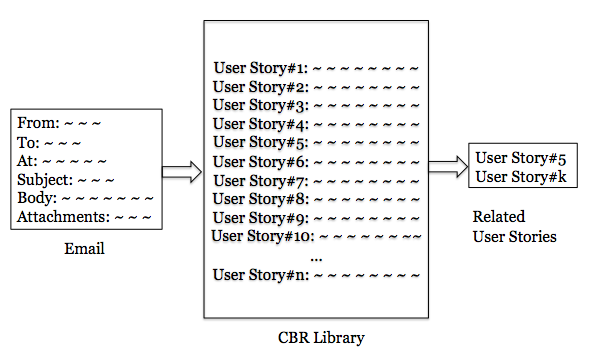
\includegraphics[width=0.6\textwidth]{CBR.png}
    \caption{CBR System Input and Output}
	\label{fig:CBR}
\end{figure*}

Figure~\ref{fig:CBR}  shows a high level view of the CBR system. A CBR system uses a library of existing cases to match against a new case. For example, Taggy has a library of existing user stories which are treated as existing cases in the CBR system. Each case is a user story, as described above, is defined by several attributes, such as, its title, description, assigned developers, customers, iteration start date and end date. Also, the data types of the attributes are different in that they include numeric date time values, symbols for emails and free text values. This library of cases is not exactly similar to a new case, an email, since the attributes are different. However, it has been discussed that it is possible to match some of the email and instant message attributes against the user story attributes. This action is performed inside the CBR system of Taggy to compute the similarity.


\subsection{Local-Global Principle}

The actual computation inside the CBR system is done following the local-global principle\cite{local_global} where it takes a two step approach, i)local similarity computation and ii) global similarity computation. Local similarity computation is confined to the similarity between only one attribute of two entities. For example, here a local similarity may be the similarity between the date of an email and the iteration start date of the user story. These local similarities are calculated in isolation from the rest of the attributes. So, the local similarity of email date and user story start date is not impacted by their local similarity for people, subject or description.

\begin{table}[at]
  \centering

  \caption{Mapping Between Email, Instant Message and User Story Attributes}
	\label{tab:mapping}
    \begin{tabular}{|p{2.5cm}|p{3cm}|p{3cm}|p{4cm}|p{2cm}|}
      \hline
      \textbf{Local Similarity} & \textbf{Email} &  \textbf{Instant Message} & \textbf{User Story} & \textbf{Type} \\
      \hline
      People & Sender, Recipients & Participants & Developer or Customer & Symbol Array\\      
      \hline
      Temporal & Email Date & Instant Message Date & Iteration start and end date & Numeric Date \\
      \hline
      Subject & Email subject & N A & Title, Description and Attachments & Free text\\
      \hline
      Body & Email Body, attachments &  Instant Message Text  & Title, Description and Attachments &  Free text\\
      \hline
    \end{tabular}

\end{table}

Table~\ref{tab:mapping} shows the adapted mapping of email and instant message attributes to user story attributes. According to this mapping, the people in email are matched against the people in user stories, so no distinction is made between the sender or recipient of an email. Similarly developers and customers of a user story are not distinguished for similarity computation. The temporal similarity again is a result of comparing the email date against a range defined by the start and end date of the iteration. And as it was stated in the assumptions, subject similarity is distinguished from the body similarity to look for important clues in the email subjects. However, in both cases the comparison is done against all the text found in a user story by looking into its title, description and attachments. This is done because the subject or body of the mail can contain similar text to any part of the user story. The same mapping applies for instant messages with two differences, i) no subject similarity is used since instant messages do not contain subject and ii) attachments from instant messages are not used.

For instant messages, this table remains same for all but the Subject similarity row, since a subject is absent in such cases. So, instant message matching requires one less local similarity measure.

On the other hand, global similarity combines the local similarities and produces a single similarity value between two entities. In this case, the global similarity combines the local similarities for people, temporal, subject and body of an email against the appropriate attributes of the user story. The combination is performed using a weighted sum of the local similarities, where the relative weight for each component is learned during the training phase.

\subsection{Similarity Function}
\label{sec:equations}
Using the aforementioned local-global principle, we adapted different equations to compute the local and global similarities as follows:

\begin{equation}
\label{eq:temporal}
S_{Temporal} =
\begin{cases}
1 & \mbox{iteration start} \le \mbox{email date} \le \mbox{iteration end}\\
0 & \mbox{if email date is within the buffer of the story's iteration} \\
-1 & \mbox{else}
\end{cases}
\end{equation}

S\textsubscript{Temporal} in Equation~\ref{eq:temporal} denotes the Temporal local similarity between an email and a user story. This equation can be interpreted as follows: if the email is sent while the user story is in development, during its iteration, then they show highest temporal similarity. However, it is also likely that an email is sent in the near past or near future of an iteration, this nearness is designated by the buffer. This buffer is set to one month. So, if an email is sent in the immediate past or future iteration of a user story, the temporal similarity is supposed to be 0. Finally, a negative score for the rest ensures emails from far past and far future are treated as highly distant in terms of temporal context. This interpretation is in alignment with the provided assumptions.

\begin{equation}
\label{eq:people}
S_{People} =
\begin{cases}
1 & \mbox{email people = user story people}\\
\frac{\# of \; common \; people}{\# of \;user \;story \;people} & \mbox{email people $\cap$ user story people $\neq$ $\emptyset$} \\
-1 & \mbox{else}
\end{cases}
\end{equation}

S\textsubscript{People} in Equation~\ref{eq:people} denotes the People local similarity between an email and a user story. This function can be interpreted as follows: if an email includes all of the people in the user story, it is highly similar in people context. Otherwise if only a few people are common, the similarity is pro-rated accordingly. Please note that, a user story is supposed to have at least one customer or customer's representative in its people context. However, when an email does not include any of the people in the user story, then it is marked as highly distant from the user story in terms of people context. In other words, this equation produces a numeric value of user story people's participation in the emails.

\begin{equation}
\label{eq:subject}
S_{Subject} = [0, 1]\mbox{, Free text similarity score (See below)}\\
\end{equation}

\begin{equation}
\label{eq:body}
S_{Body} = [0, 1]\mbox{, Free text similarity score (See below)}\\
\end{equation}

S\textsubscript{Subject} and S\textsubscript{Body} represents the free text similarity score for the two attributes. The values are found form the full text search engine and can be anything between 0 and 1 as shown in Equation~\ref{eq:subject} and Equation~\ref{eq:body}. Computing the textual similarity between two free format texts is in itself a research topic and beyond the scope of this thesis. However, Taggy used an industry standard open-source full text search engine called Lucene to produce this score\cite{lucene}. The search engine uses a Vector Space Model \cite{a_vector_space} to compute the similarity between two free text documents. This model first defines the index of a free text document in terms of a vector that captures the frequency and relative weight of each term in the document. Next, an inner product of two such vectors is used to produce their similarity. Also, to compare the similarity of a document against a library of documents, the similarity results are normalized for the length of the documents. This approach is highly scalable since the similarity computation of two different documents is turned into simple vector computation. Also, the generation of the vectors can benefit from using synonyms, stop words and other language specific stems. Very high-traffic applications have used this approach to facilitate full text search. For example, Twitter, a popular micro-blogging site that serves 12000 searches/second, at the time of writing of this thesis is using this search engine \cite{twitter_lucene}. However, the text of an email is very unlikely to be exactly same as a user story. So, it is not generally expected that Lucene will return a value of 1 in such case. In fact, during the evaluation I have found that email texts that are highly similar to user story texts had Lucene similarity score of 0.4-0.5. Based on this finding, S\textsubscript{Subject} and S\textsubscript{Body} are assigned a value of 1 if Lucene score is great than or equal to 0.4. Otherwise, the values are pro-rated accordingly. For example, a Lucene score of 0.2 for a subject is actually converted to S\textsubscript{Subject} = 0.5 as a result of this pro-rating.

%http://engineering.twitter.com/2010/10/twitters-new-search-architecture.html                                                       
The choice of the above equations are based on the experience from looking into the data. However, the software is trained to learn the relative weights of these local similarities. The learning process adjusts the relative weights so that the global similarity computation minimizes the number of wrong decisions.

Next, the global similarity function combines the local similarities from the above equations using the following formula:

\begin{equation}
	\label{eq:global}
S_{Global} = \frac{W_{Temporal} * S_{Temporal} + W_{People} * S_{People} + W_{Subject} * S_{Subject} + W_{Body} * S_{Body}} {W_{Temporal} + W_{People} + W_{Subject} + W_{Body}}\\
\end{equation}

where,
\begin{equation}
	\label{eq:w_temporal}	
W_{Temporal} = \mbox{relative weight of temporal similarity}
\end{equation}      

\begin{equation}   
		\label{eq:w_people}
W_{People} = \mbox{relative weight of people similarity}
\end{equation}

\begin{equation}     
		\label{eq:w_subject}
W_{Subject} = \mbox{relative weight of subject similarity}
\end{equation}

\begin{equation}     
		\label{eq:w_body}
W_{Body} = \mbox{relative weight of body similarity}
\end{equation}

As Equation~\ref{eq:global} shows, the global similarity is a weighed sum of the local similarity values. But the relative weights are not known a priori. Instead, Taggy learns the relative weights for the different components so that it can potentially reflect the relative importance of each of the component based on a training data set. Using a weighted sum provides transparency about the decision-making logic inside Taggy.
	
\subsection{Learning Relative Weights}	
\label{sec:learning}
Taggy uses a Reinforcement Learning approach to learn the relative weights of the different components to compute a measure of global similarity \cite{reinforcement_learning}. The learning algorithm is designed to adapt the relative weights of the local similarity measures based on the feedback from its decision being correct or incorrect.

Since the local similarity measures participate in the process of global similarity computation, their relative weights are adjusted based on their contribution to a correct or incorrect decision. For example, if a decision is correct and the people similarity score is positive, then the relative weight of people similarity score, as seen in Equation~\ref{eq:w_people}, is increased by 1. On the other hand, if the decision is correct but the people similarity score is negative, then it is punished by lowering the weight by 1. So, depending on the decision of an individual component and the final outcome, the relative weights are adjusted accordingly. This process continues unless all training data are exhausted or the adaptation converges.

However, it is important to initialize the relative weights of the local similarity measures based on a meaningful foundation so that the entry point is not absolutely random. This is done by running the training data for each local similarity while keeping the others in isolation - for example, trying to auto-tag emails with user stories solely based on their people similarity and doing the same for other local similarity components. Once this is done, the number of correct decisions made by each component provides a rough estimate of its relative importance over another component. These numbers of correct decisions are normalized to produce the initial relative weights of the four components, namely, people, temporal, subject and body similarity measures.

Once the initial weights are found, the following algorithm is used to implement the reward-punishment scheme of the reinforcement learning approach:

\pagebreak
\begin{verbatim}
date_weight     = initial_date_weight
people_weight   = initial_people_weight
subject_weight  = initial_subject_weight
body_weight     = initial_body_weight

for all_training_emails do |email|
   result = find_most_similar_user_stories(email)
   is_correct = result.guessed_stories == email.actual_stories
	
   is_date_similar    = result.date_similarity >= 0
   is_people_similar  = result.people_similarity >= 0
   is_subject_similar = result.subject_similarity >= 0.5
   is_body_similar    = result.body_similarity >= 0.5

	 #Adjust temporal similarity weight
   if (is_correct and is_date_similar) or 
      (!is_correct and !is_date_similar) then
    date_weight = reward(date_weight)
   else
    date_weight = punish(date_weight)
   end

   #do the same for people, subject and body similarity
		. . .		
   end
end
\end{verbatim}
This algorithm shows the reward-punishment in action for the temporal similarity weight. This essentially rewards the local similarity weight of a component that contributes in making a correct decision while punishes the one that influences a wrong decision. This reward-punishment continues unless all training emails are seen. Also, it is possible to stop if this converges to a point when adding new emails do not alter the relative weights. However, as with most machine learning techniques, the usefulness of this learning is dependent on the quality and quantity of the training data. As shown before, Taggy's Learner component implements this algorithm. Once the learning is done, relative weights are tuned to auto-tag emails with user stories. This same algorithm can be used to learn relative weights for instant messages, where the subject is missing.

The choice of this reward-punishment scheme makes it transparent, as one can easily follow the changes in the relative weights based on the logic. Other machine learning approaches such as different variations of back propagation algorithm could also be utilized instead of this one.

\section{Architecture}
Taggy is composed of a number of different components to support the workflow as outlined in the previous section. The key components of Taggy is depicted at Figure~\ref{fig:architecture}. Next, the details about each component from the figure is discussed following a bottom-up approach.

\begin{figure*}[!h]
	\centering
	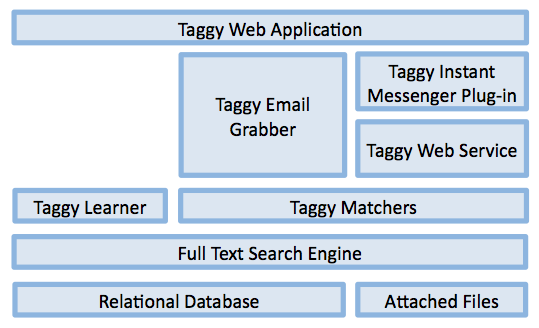
\includegraphics[width=0.8\textwidth]{architecture.png}
    \caption{Taggy Components}
	\label{fig:architecture}
\end{figure*}

\begin{enumerate}
	\item \textbf{Relational Database.} This relational database component persists the agile project related information. To address the concern of auto-tagging, this database keeps the following information:
		\begin{itemize}
			\item People. People information includes a person's name, email address and instant messenger id, if any. Also, a project vs. people mapping is stored.
			\item Iteration. Iterations, defined by start and end dates, are also saved.
			\item User story. Each user story may have a title and description. Also, if the story is planned, then information about its iteration and assigned people are stored in the database.
			\item Email. The database also stores the subject and content of the emails with a link to sender and recipients if they are found in the people information. If the email is tagged with a user story, then this information is kept in the database as well. In case the the database does not include some or all of the emails found in sender and recipients of an email, the information is still stored but no mapping against existing users are made for the missing email addresses. So, missing email addresses do not contribute to the people similarity computation.
			\item Instant Message. Similar to emails, the database stores the instant messages and their tagging information.
		\end{itemize}

	 \item \textbf{Attached Files.} Attached Files is a simple file system storage where all attachments are kept. An attachment may be part of a user story definition or can be extracted from an email.
	
	 \item \textbf{Full Text Search Engine.} This component produces full text index from contents found in user stories, emails and their associated attachments. This is a third party component called Lucene that can handle synonyms and language specific stems \cite{lucene}. The attached files are only indexed for full text search if it would be meaningful - for example, image files are not indexed where PDF file contents are.
	
	\item \textbf{Taggy Matchers.} This is the core component of Taggy that produces the auto-tagging, i.e. the similarity related computations are done inside this component. There are two matchers inside Taggy: email matcher and instant message matcher. These two matchers share some common computation logic. However, instant messages don't have subjects as found in emails and as a result, the two matchers use different relative weights and minimum threshold similarity scores to auto-tag. The matchers depend on the full text search engine and the relational database to lookup required data.
	
	\item \textbf{Taggy Learner.} As discussed before, Taggy requires training to learn different parameters. This component takes care of the learning process. During learning the Learner uses the Matcher to auto-tag an email and depending on the outcome, it may learn the parameters of interest. Once the learning is complete, the learner sets the relative weights to be used in the Matcher. So, the core part of auto-tagger is a mix of its Learner and Matcher components.
	
	\item \textbf{Taggy Email Grabber.} The Email Grabber component works as a background process that periodically checks for incoming emails in any of the project emails. If it finds one, it reads the email, saves a copy in the relational database as well as downloads the attachments into Attached Files. Next, the text contents are all indexed through the Full Text Search Engine. With this data persisted, it invokes the Matcher component to auto-tag the email against the relevant user stories. This handles the email intake process to Taggy.
	
	\item \textbf{Taggy Web Service.} Taggy exposes a web service so that an instant messenger plugin can push instant messages to Taggy.
	
	\item \textbf{Taggy Instant Messenger Plug-in.} This component is installed as a plug in to an instant messenger. Once activated, this component sends instant messages to the Web Service Component.
	
	\item \textbf{Taggy Web Application.} The web application provides interfaces for manipulating everything in Taggy. For example, one can browse a user story and see all related emails and instant messages or vice versa. Also, one can search through all the contents, including the attachments. In a nutshell, this is a light-weight agile project management tool with the additional feature that it auto-tags emails and instant messages.
\end{enumerate}

\subsection{Email Matching}
Once the relative weights are learned, Taggy can match emails against user stories based on the trained system. This process essentially starts with grabbing email and saving it. A developer or customer sends out emails about the project and copies to Taggy using CC: feature. While saving, a lookup is performed to see if the email addresses present in the sender, recipients and CC: match against any of the existing users' record in Taggy's relational database for the project. If found, the users are linked with the emails. Next, the email matcher of the Taggy Matchers component is asked to look for relevant user stories in the database.

\begin{figure*}[tb]
	\centering
	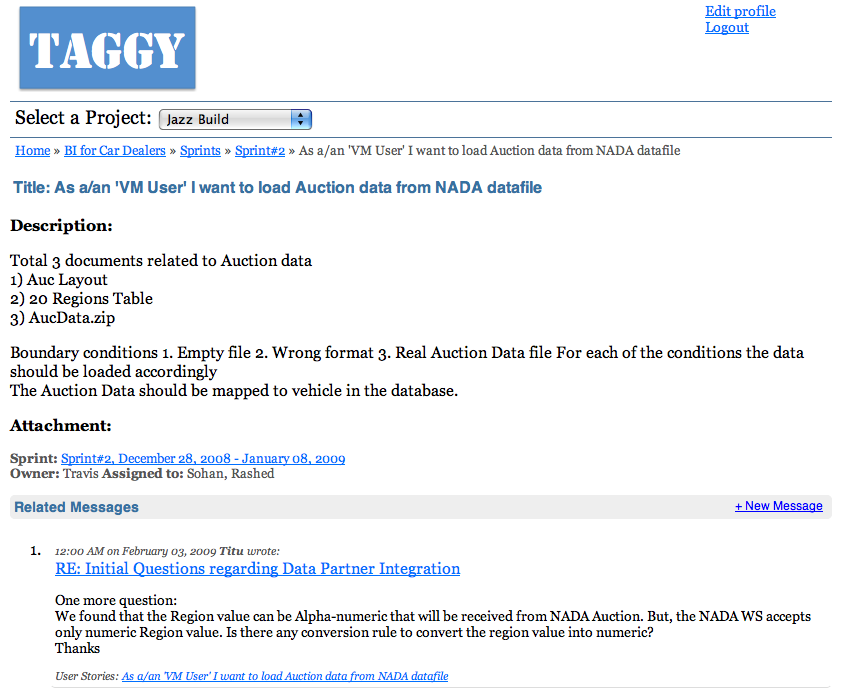
\includegraphics[width=\textwidth]{taggy_user_story.png}
	\floatstyle{boxed} 
    \caption{Taggy Screenshot - Showing User Story and Related Emails}
	\label{fig:taggy_user_story}
\end{figure*}

	
\begin{figure*}[tb]
	\centering
	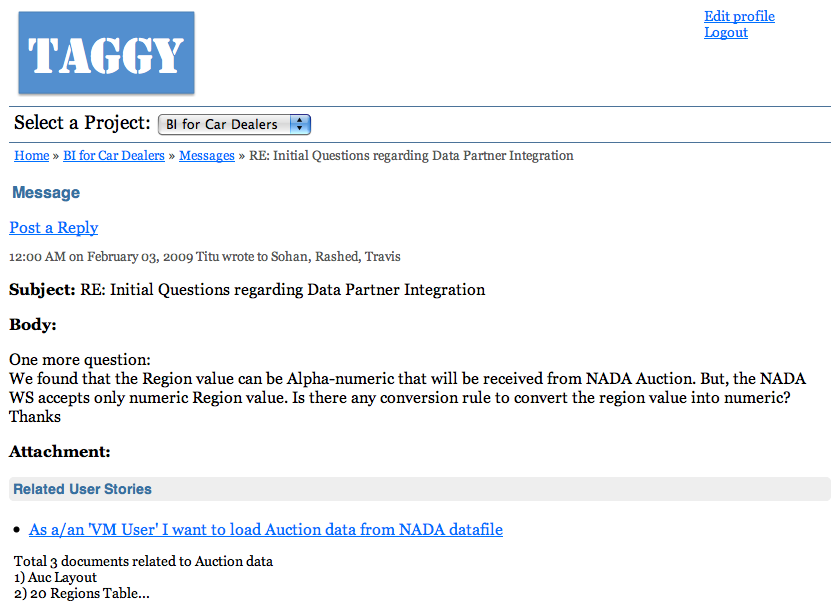
\includegraphics[width=\textwidth]{taggy_email.png}
    \caption{Taggy Screenshot - Showing Email and Related User Stories}
	\label{fig:taggy_email}
\end{figure*}

To an end user of Taggy, the outcome of auto-tagging is as shown in Figure~\ref{fig:taggy_user_story} and Figure~\ref{fig:taggy_email}. So, while browsing user stories, one can see the related emails or vice versa. This same outcome is found for instant messages as well. So, this email matching is responsible for ``matchmaking'' among the emails and user stories based on their context and text similarity.

The email matcher filters out user stories so that user stories from far past or future are discarded. Next, it computes the local similarity measures and combines them  to produce global similarity values. The ones that show a global similarity above a threshold, survives as the potential candidates for auto-tagging. Based on user preferences, the email is auto-tagged against the top n user stories, where n is any number greater than or equal to 1. The following code fragment shows these steps:

\pagebreak              
\begin{verbatim}
def	find_most_similar_user_stories(email, n)
  nearby_user_stories = UserStory.planned_nearby(email.date)

  if nearby_user_stories
    temporal_scores = find_temporal_scores(nearby_user_stories, email.date)
    people_scores 	= find_temporal_scores(nearby_user_stories, email.people)
    subject_scores 	= find_subject_scores(nearby_user_stories, email.subject)
    email_text 			= email.body_with_attachment
    body_scores 		= find_body_scores(nearby_user_stories, email_text)

    global_scores = compute_global_scores(relative_weights, temporal_scores, 
																people_scores, subject_scores, body_scores)

    global_scores_above_threshold =  discard_under_threshold_scores(global_scores)

    if global_scores_above_threshold.present?
    	return global_scores_above_threshold[0..(n-1)]
    end
		
  end
	
  return blank
	
end
\end{verbatim}

The different similarity computations in the email matcher are carried out using the Equation~\ref{eq:temporal}, Equation~\ref{eq:people}, Equation~\ref{eq:subject}, Equation~\ref{eq:body} and Equation~\ref{eq:global}. As shown in the code fragment, one can configure Taggy email matcher to auto-tag with the top n number of top matches. Having n greater than 1 helps to identify cases when an email is potentially relevant about two or more user stories. However, in some teams this situation may be different where most of the time the communication is just about a single user story. So, this configuration will help them to tune Taggy according to their communication patterns. Although not implemented, Taggy could also learn this parameter, n, based on the training data. If the the training data shows that most emails only discuss a single user story, it may only choose to show the most relevant story or adjust this number based on the trend.

This matching algorithm is run in the same background process as that of the Email Grabber. Because of the filtering step, Taggy has a reduced search space to deal with. For example, when filtering is used, in a project with 695 user stories, it took an average of 1.16 seconds per email for auto-tagging. However, the to do the same without the filtering it took an average of 2.12 seconds on the same data. Although this improves speed, it may produce a wrong decision if a distributed agile team chooses to discuss about user stories from the distant past in the emails. In such cases, the definition of ``distant'' needs to be adjusted accordingly. In the implementation of Taggy, anything beyond immediate past and future month of an iteration is treated as ``distant'' based on the observation from training data.

\subsection{Instant Message Matching}
The instant message matcher is implemented using the same approach, since we can find similar people and temporal context from instant messages as well. As discussed earlier, the intake process is different for instant messages, which uses a Taggy web service to push chat messages from a Taggy Instant Messenger Plug-in. The actual similarity computation in case of instant messages omits the subject similarity and applies a different relative weight scheme. The threshold is also adjusted accordingly.







\section{An Illustrative Example}	
Now that the details about Taggy's internals are provided, the following illustrative example will demonstrate Taggy in action.

First, a project's backlog is populated with user stories. This backlog has stories from different iterations. For brevity, a shortened backlog is given at Table~\ref{tab:backlog}:

\begin{table}[h!]
  \centering
  \caption{An Example Product Backlog}
    \begin{tabular}{|p{0.5cm}|p{1.7cm}|p{1.2cm}|p{1.2cm}|p{9cm}|}
      \hline
      \textbf{\#} & \textbf{Iteration} & \textbf{Cust- omer} & \textbf{Deve- loper} & \textbf{Description}\\
      \hline
		1 & \#1, Dec 14-25, 2008 & C1 & D1 & As a/an `VM User' I want to add/edit/view dealer account profile so that VM can earn revenue from charging a monthly subscription fee.
			Dealers will have three contacts: Billing, General Manager and Owner. Also, there will be a primary and secondary contact. More information is attached.\\
      \hline
		2 & \#1, Dec 14-25, 2008 & C1 & D2 & As a/an `VM Admin' I want to add/edit/view VM users. 
		Administrator must be able to see username but not password VM Users will be one of inside rep and outside rep. 
		Required fields and more information are attached...\\
	  \hline
		3 & \#2, Dec 28, 2008-Jan 08, 2009 & C1 & D1 & As a/an `VM user' I want to load DMV data from Experian from a CSV/Excel file into VM database. Sample data attached.\\
	  \hline
		4 & Not Assigned & C1 & D1 & As a/an `VM User' I want to activate and deactivate a dealer\\
	  \hline
    \end{tabular}
		\label{tab:backlog}
\end{table}

This backlog has 4 user stories. The stories are assigned to two developers, D1 and D2, and only one customer C1. Also, this backlog contains stories from Iteration\#1, December 14-25, 2008 and Iteration\#2, December 28, 2008 to January 8, 2009. Also, the user story\#4 is not yet planned for any iteration. In an agile team, this list is likely to be longer with more user stories, iterations, developers and customers. However, for the sake of an example, this small backlog serves the purpose.

Now, developer D1 needs to get a clarification from the customer C1 while working on a user story at the start of iteration\#1. This is asked using the email as shown below:

\begin{quote}
	\textbf{To:} C1\\
	\textbf{From:} D1\\
	\textbf{CC:} project@Taggy\\
	\textbf{Date:} Dec 14, 2008\\
	\textbf{Subject:} Initial Questions on \textbf{Dealer setup}\\
	\textbf{Body:}\\
	Please clarify the following questions regarding dealer setup data-\\
	1. Is it ok to assume that the billing, GM and Owner contacts of a dealer will also contain username/passwords. Note that, the main and secondary contacts as well as the Used car manager contact contain user name/passwords.\\
	2. What data should we collect for Physical Address and Mailing Address of a dealer? Is it free text? Or collected as fields street1, street2, city, state, zip, country?\\
	3. Is it possible that for a dealer both an inside and outside salesman is assigned?\\
	4. Apart from the name and pricing, is there any other field associated with the ``program'' {main/platinum} information?\\
	5. What is meant by the ``Location'' field of the outside VM Rep?\\
	6. Is it possible to provide us with a sample input data that will be used to set up an inside/outside VM user's commission? Please provide examples of default, bonus, retention and special commissions.\\
	7. What are the required fields of all the dealer setup fields?\\
	8. The Business Address is mentioned twice under the 5.6.1.5 - do we need to capture two business addresses?
	\\
\end{quote}

Please note that this email has a CC: to project@Taggy. So, Taggy will be able to read the contents of this email. As shown in the email matcher, Taggy will try to auto-tag the email with the existing user stories based on context and text relevance. While doing so, the local and global similarities are computed as shown in Table~\ref{tab:similarity}:

\begin{table}[h!]
  \centering
  \caption{Similarity Scores}
    \begin{tabular}{|p{1.2cm}|p{1.5cm}|p{1.2cm}|p{1.2cm}|p{1.2cm}|p{1.4cm}|p{1.4cm}|p{1.1cm}|p{1.1cm}|p{1.2cm}|}
      	\hline
		\textbf{Story \#} & \textbf{Tempo-ral Sim.} & \textbf{Tempo-ral. Wgt.} & \textbf{People Sim.} & \textbf{People Wgt.} & \textbf{Subject Sim.} &\textbf{Subject Wgt.} & \textbf{Body Sim.} &\textbf{Body Wgt.} &\textbf{Global Sim.}\\
		\hline
		1 & 1 	& \multirow{4}{*}{28.6} & 1 	& \multirow{4}{*}{20.2}	& 0.6 & \multirow{4}{*}{34.4}	& 0.4 & \multirow{4}{*}{16.8}	& \textbf{0.76}\\
		2 & 1 	&  & 0.5 	&  	& 0.4 	&	& 0.25	&	& 0.57\\
		3 & 0 	&  & 1 		& 	& 0 		& & 0.2	&	& 0.24\\
		4 & -1 	&  & 1 		& 	& 0.3 	& & 0.3	&	& 0.07\\
		\hline
	\end{tabular}
	\label{tab:similarity}
\end{table}  

Here, similarity scores are computed based on the similarity equations. For example, user story\#1 has a people similarity score of 1, since all people in the story, C1 and D1, are present in the email. On the other hand, user story\#2 has a people similarity score of 0.5 since only one (C1) of the two people from the user story is found in the email. The values for other similarity measures can also be traced following the respective equations.

From the above table we see that Story \#1 is the most similar story to the given email with a similarity score of 0.76. This is greater than the threshold of 0.58 (details discussed in Chapter~\ref{ch:evaluation}) and thus the system auto-tags the email with Story \#1. However, the other stories are not considered as related as those failed to reach the threshold similarity score.

In this example the email is auto-tagged with user story\#1. However, if the threshold is set to a lower value or there was another user story with similar profile to user story\#1, Taggy could recommend more than one auto-tagging. On the other hand, it could simply ignore auto-tagging with any user story if another email was too irrelevant for the given backlog.

\section{Implementation Details}
Figure~\ref{fig:implementation} shows the implementation frameworks for the different architectural components.

\begin{figure*}[!h]
	\centering
	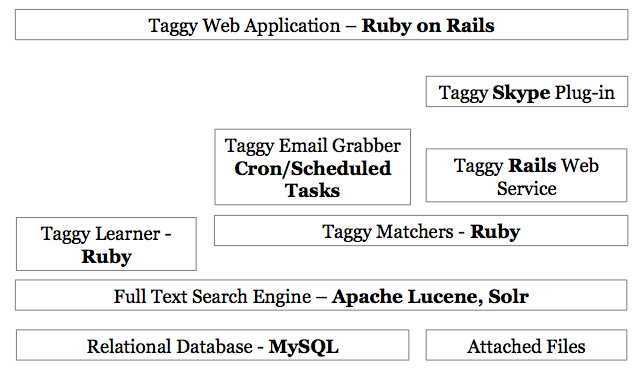
\includegraphics[width=0.8\textwidth]{Implementation.png}
    \caption{Taggy Implementation Details by Component}
	\label{fig:implementation}
\end{figure*}


As with any software solution, the implementation of Taggy was based on available programming languages and platforms. The core Taggy components, the Learner and Matcher, are developed using the Ruby programming language \cite{ruby}. The web application is also developed using the open-source Ruby on Rails web framework \cite{ruby_on_rails}. The choice of this framework was based on my prior experience as well as its support for producing quick data-backed web application development.

The full text search is served by Apache Lucene \cite{lucene}. This open-source search engine is widely used across the web to facilitate full-text search. In a previous implementation of Taggy, I used Microsoft SQL Server Full-Text Search Engine \cite{auto_tagging, sql_server}. But Lucene was chosen because of its ability to index rich text files such as Word Documents, and PDF files. Also, Lucene can be configured to support synonyms, language stems and comes with out-of-the-box support for full-text search using several languages. However, the architecture of Taggy allows the replacement of this engine by another one without impacting the rest of the system.

To communicate with Lucene, a web service wrapper called Solr is used \cite{solr}. Solr's RESTful web API provides easy access to Lucene indexing and querying from other languages, such as Ruby. Solr and Lucene can index the contents from rich documents such as PDF files, Word documents and Spreadsheets. This feature was used to index both user story and email attachments alongside their primary contents.

Since most project management tools support full-text search anyway, this indexing is not likely an additional burden applied by Taggy. However, understandably the index size of Taggy may grow if a team frequently uses emails and instant messages, which is otherwise not captured by most of the project management tools.

For capturing instant messages, a Skype plugin is developed using the Skype4Py library \cite{skype4py}. The plugin can be turned on/off by the click of a button. When activated, it copies the chat messages with meta information and sends this data to the web service. Skype was picked because its use as a popular instant messenger service in software knowledge sharing \cite{how_did_we}. Also, it offers a suite of features that are used by distributed agile teams such as group chat, group video conferencing, and screen sharing. A similar plugin can be developed for other instant message services if supported by the platform.

The background process for the email grabber can be run using Cron jobs on Unix based platforms or scheduled tasks on Windows based platforms \cite{cron, scheduled_tasks}. These scheduling tools can be configured to look for new incoming emails in preferred intervals starting from once every second to any realistic period.

Taggy uses a MySQL relational database server to store the data. This can be replaced by any relational database supported by ActiveRecord, which includes MySQL, Oracle, Microsoft SQL Server, SQLite, Derby etc \cite{active_record}. Also, it is possible to use any data storage without using ActiveRecord at all as long as Taggy gets data with a similar schema.

As of hardware platform, Taggy does not impose any special requirements compared to other agile project management tools.
